\subsection{Layer Operating System}
The front-end, like the entire application, will be run on the browser and will therefore run on any operating system.

\subsection{Layer Software Dependencies}
The entire application will depend on Bootstrap, and the React library.

\subsection{Login Subsystem}
The Login Subsystem will will provide an interface for user to login into the application. Users will be able to login with their email and password credentials or their Google accounts.

\begin{figure}[h!]
	\centering
 	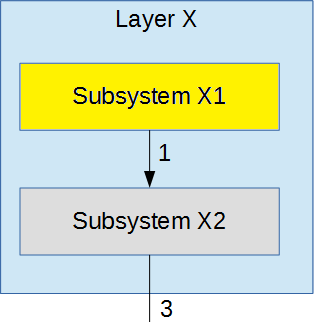
\includegraphics[width=0.60\textwidth]{images/subsystem}
 \caption{Example subsystem description diagram}
\end{figure}

\subsubsection{Subsystem Software Dependencies}
The Login Subsystem will require a consistent connection to the applications database in order to login with their email and password credentials. For a user to login with their Google accounts, the application will depend on the GoogleLogin library.

\subsubsection{Subsystem Programming Languages}
The Login Subsystem will be developed using, React.js, HTML, and CSS.

\subsubsection{Subsystem Data Processing}
If the user logs in using their email and password, they will enter their credentials in the respective places and click the login button. Upon the login buttoin being pressed, the Login Subsystem will send the user's credentials to the Query Manager in the backend layer. If the Login Subsystem receives a success signal, then the user will be redirected to the Home Page. If the Login Subsystem receives a failure signal, the Login Subsystem will display a failure message and prompt the user to re-enter their credentials.

If the user decides to login with their Google account, they will select the Google login button. The Login Subsystem will then call on the GoogleLogin API which users will login with. If the login is successful, the Login Subsystem will redirect the user to the Home Page. If the login fails, the user will be given an error message and prompted to re-enter their credentials.

%------------> Register 
\subsection{Register Subsystem}

\begin{figure}[h!]
	\centering
 	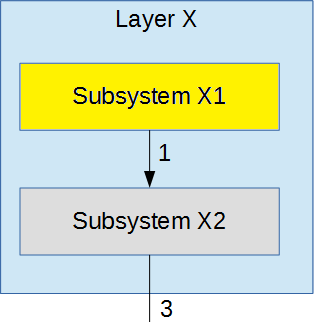
\includegraphics[width=0.60\textwidth]{images/subsystem}
 \caption{Example subsystem description diagram}
\end{figure}

\subsubsection{Subsystem Software Dependencies}

\subsubsection{Subsystem Programming Languages}
The Login Subsystem will be developed using, React.js, HTML, and CSS.

\subsubsection{Subsystem Data Processing}

%------------> Shopping List
\subsection{Shopping List Subsystem}

\begin{figure}[h!]
	\centering
 	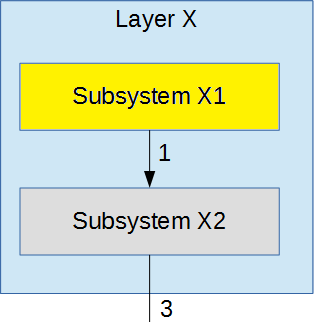
\includegraphics[width=0.60\textwidth]{images/subsystem}
 \caption{Example subsystem description diagram}
\end{figure}

\subsubsection{Subsystem Software Dependencies}

\subsubsection{Subsystem Programming Languages}
The Login Subsystem will be developed using, React.js, HTML, and CSS.

\subsubsection{Subsystem Data Processing}

%------------> Recipes
\subsection{Recipes Subsystem}

\begin{figure}[h!]
	\centering
 	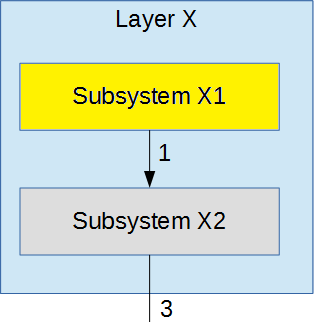
\includegraphics[width=0.60\textwidth]{images/subsystem}
 \caption{Example subsystem description diagram}
\end{figure}

\subsubsection{Subsystem Software Dependencies}

\subsubsection{Subsystem Programming Languages}
The Login Subsystem will be developed using, React.js, HTML, and CSS.

\subsubsection{Subsystem Data Processing}

%------------> Meal Plan
\subsection{Meal Plan Subsystem}

\begin{figure}[h!]
	\centering
 	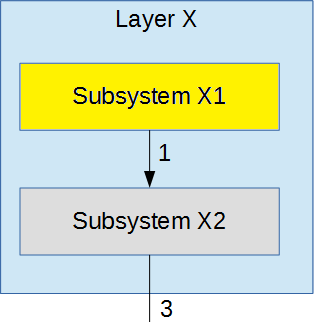
\includegraphics[width=0.60\textwidth]{images/subsystem}
 \caption{Example subsystem description diagram}
\end{figure}

\subsubsection{Subsystem Software Dependencies}

\subsubsection{Subsystem Programming Languages}
The Login Subsystem will be developed using, React.js, HTML, and CSS.

\subsubsection{Subsystem Data Processing}

%------------> Shop
\subsection{Shop Subsystem}

\begin{figure}[h!]
	\centering
 	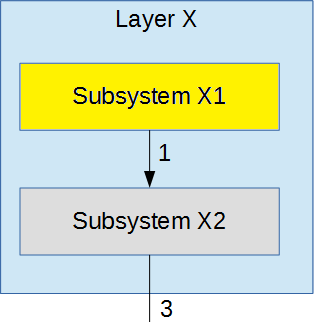
\includegraphics[width=0.60\textwidth]{images/subsystem}
 \caption{Example subsystem description diagram}
\end{figure}

\subsubsection{Subsystem Software Dependencies}

\subsubsection{Subsystem Programming Languages}
The Login Subsystem will be developed using, React.js, HTML, and CSS.

\subsubsection{Subsystem Data Processing}


